%! Author = borisdeletic
%! Date = 08/05/2023

% Preamble
\documentclass[11pt]{article}

% Document
\begin{document}

    \section{Bayesian Inference}\label{sec:bayesian_inference}
    Bayesian inference is a robust analytic framework which allows the construction of predictive models $\mathcal{M}$
    in the context of some dataset $\mathcal{D}$.

    The \emph{likelihood} is defined as the probability of observing the data given a specific parameter choice $\theta$
    \begin{equation}\label{eq:likelihood}
        p(\mathcal{D} | \theta, \mathcal{M}) \equiv \mathcal{L}(\theta).
    \end{equation}
    A Bayesian model must also specify it's distribution of parameters before any data is known.
    This is termed the \emph{prior}, defined by
    \begin{equation}\label{eq:prior}
        p(\theta|\mathcal{M}) \equiv \pi(\theta).
    \end{equation}
    The \emph{evidence} is the distribution of observed data marginalised over the parameters, defined as
    \begin{equation}\label{eq:evidence}
        p(\mathcal{D} | \mathcal{M}) \equiv \mathcal{Z} = \int{\mathcal{L}(\theta) \pi(\theta) d\theta}.
    \end{equation}
    The evidence, or sometimes \emph{marginalised likelihood}, is an important quantity which provides a measure
    on the quality of a model $\mathcal{M}$.

    By using Bayes' Theorem~\cite{bishop2006}, the distribution of parameters $\theta$ given our model and data
    can be written in terms of the quantities
    \begin{equation}\label{eq:bayes_theorem}
    \begin{aligned}
        p(\theta | \mathcal{D}, \mathcal{M}) &=
            \frac{p(\mathcal{D} | \theta, \mathcal{M}) p(\theta|\mathcal{M})}{p(\mathcal{D} | \mathcal{M})}, \\
        \mathcal{P}(\theta) &= \frac{\mathcal{L}(\theta) \pi(\theta)}{\mathcal{Z}},
    \end{aligned}
    \end{equation}
    where $\mathcal{P}(\theta)$ is termed the \emph{posterior}.
    The posterior is the distribution of parameters $\theta$ after taking the data into account.

    An intuitive relationship between these quantities is that a model where the \emph{prior} more closely
    resembles the \emph{posterior} will have a greater \emph{evidence}~\cite{mackay2003}.

    Calculating the posterior is in the domain of \emph{parameter estimation}, which is often a very difficult task
    to solve analytically.
    For high-dimensional problems, we therefore resort to computationally estimating the distribution by sampling
    from the posterior using Markov-Chain Monte-Carlo techniques~\cite{gupta2014comparison, delmoral2013mean}.

    Examples of such sampling algorithms include Metropolis-Hastings~\cite{Metropolis_OG},
    Slice sampling~\cite{neal2003slice}, and Hamiltonian Monte Carlo~\cite{HMC_Duane, neal1996monte}~\ref{sec:hamiltonian_monte_carlo}.

    \section{Nested Sampling}\label{sec:nested_sampling}
    Nested sampling is an algorithm which simultaneously computes
    the evidence and posterior~\cite{Skilling2006, Handley_polychord, NS_Review_2022}.
    For a set of parameters $\theta$ with dimension $D$, calculating the evidence through direct evaluation of the
    high-dimensional integral~\ref{eq:evidence} becomes exponentially more expensive as $D$ is increased.

    We define the \emph{prior volume} as the fraction of prior contained within an iso-likelihood contour
    \begin{equation}\label{eq:prior_volume}
        X(\lambda) = \int_{\mathcal{L}(\theta)>\lambda} \pi(\theta) d\theta.
    \end{equation}
    Using a change of variable we write the evidence as a one-dimensional integral more feasible to calculate
    \begin{equation}\label{eq:evidence_ns}
        \mathcal{Z} = \int_0^1 {\mathcal{L}(X)} dX
    \end{equation}

    Nested sampling introduces a population of $n_{\text{live}}$ \emph{live points} in the parameter space which are sorted
    by likelihood.
    These points are then iteratively updated to compress around the peaks of the posterior distribution.

    Initially, $n_{\text{live}}$ points are sampled from the prior $\pi(\theta)$.
    At each iteration $i$, the point with the lowest likelihood $\mathcal{L}_i$ is deleted and moved to the set
    of \emph{dead points}.
    A new live point is then generated from the prior, subject to the hard constraint that its likelihood is
    greater than $\mathcal{L}_i$.

    The prior volume on average will contract by a factor $n_{\text{live}}/(n_{\text{live}}+1)$ with each dead point, such that the
    expected prior volume at iteration $i$ will be
    \begin{equation}\label{eq:exp_prior_volume}
        \langle X_i \rangle = \left( \frac{n_{\text{live}}}{n_{\text{live}} + 1} \right)^i \approx e^{-i/n_{\text{live}}},
    \end{equation}
    thus compressing exponentially for large $n_{\text{live}}$.
    Each dead point has a likelihood $\mathcal{L}_i$, a set of parameters $\theta_i$, and a prior mass $X_i$, which can
    be used to estimate the evidence and posterior.

    \begin{figure}[t!]
        \center
        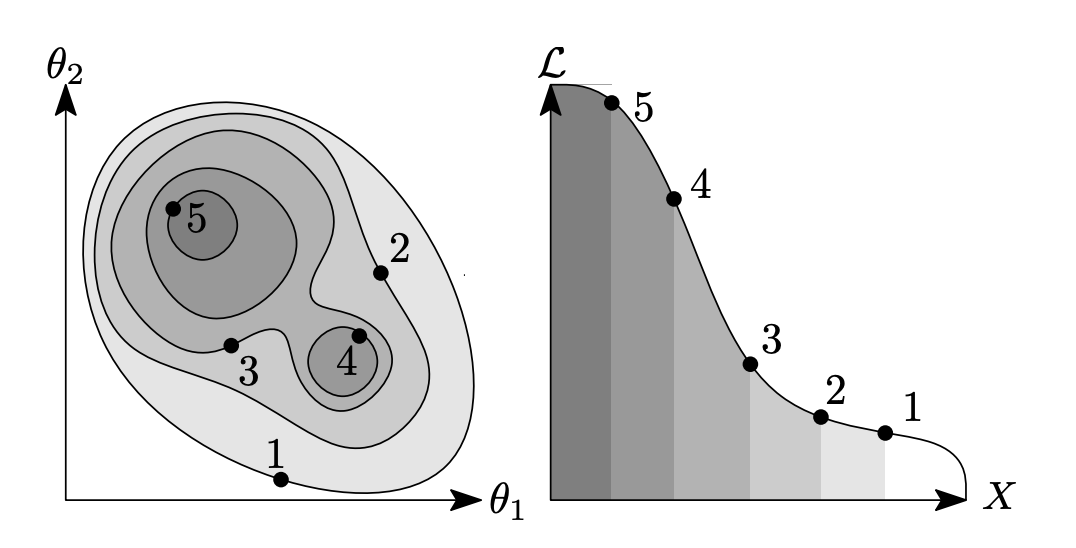
\includegraphics[width=\linewidth]{../figures/NestedSamplingPolychord}
        \caption{
            Nested sampling prior volume transformation. Left: Five sequentially higher iso-likelihood contours of a
            two-dimensional bimodal likelihood function $\mathcal{L}(\theta)$. Each contour encloses a smaller fraction
            of the prior volume $X$. Right: Likelihood $\mathcal{L}(X)$ as a function of enclosed volume $X$. The
            Bayesian evidence is the area under the curve.~\cite{Handley_polychord, Handley_2015}
            (figure and caption used from paper).
        }\label{fig:nested_sampling}
    \end{figure}


\subsection{Evidence and Parameter Estimation}\label{subsec:evidence_param_estimation}
    We can use the dead points generated by the algorithm to computationally estimate the evidence.
    Approximating the integral~\ref{eq:evidence_ns} using the trapezoid rule, we write
    \begin{equation}\label{eq:evidence_estimation}
        \mathcal{Z} \sum_{i \in \text{dead}} w_i \mathcal{L}_i,
    \end{equation}
    where $w_i = (X_{i-1} - X_{i+1})/2$ is the weight factor estimating the change in prior volume per iteration.
    Further discussion of this estimation and the associated errors can be found in
    Handley et al.~\cite{Handley_2015, NS_Review_2022}.

    We can also use the dead points as samples from the posterior.
    Given the $i$-th sample is assigned an importance weighting $w_i$, the posterior samples are
    \begin{equation}\label{eq:posterior_ns}
        p_i = \frac{w_i \mathcal{L}_i}{\mathcal{Z}} \propto w_i \mathcal{L}_i.
    \end{equation}
    Most MCMC algorithms are not concerned with the evidence and therefore only generate un-normalised posterior samples.

\subsection{Termination criteria}\label{subsec:termination_criteria}
    The stopping criteria for nested sampling as suggested by Handley et al.~\cite{Handley_2015}, is determined by
    the remaining evidence in the live points.
    We terminate the algorithm once the evidence in the live points is a small fraction of the total accumulated evidence,
    determined by the precision criterion $\mathcal{Z}_{\text{live}} / \mathcal{Z}$.

    The remaining evidence can be estimated by assuming all the live points have the same prior volume at iteration $i$
    \begin{equation}\label{eq:remaining_evidence}
    \mathcal{Z}_{\text{live}} \approx \langle \mathcal{L} \rangle_{\text{live}} X_i.
    \end{equation}
    As this approximation will overestimate the live evidence, this will generally not cause early stopping of the algorithm.
    Further discussion of this can be found in Feroz~\cite{Feroz_2009}, Handley~\cite{Handley_2015}, and
    Keeton~\cite{keeton2011statistical}.

    \subsection{Choosing $n_{\text{live}}$}\label{subsec:ns_termination}
    The input parameter for the number of live points $n_{\text{live}}$, has a significant impact on the quality of results generated.
    More live points will increase the precision for the estimate of prior volume~\ref{eq:prior_volume} and force more
    iterations to contract onto the posterior, however more computational time will be required to complete the algorithm.

    The remaining evidence $\mathcal{Z}_{\text{live}}$ can be used to calculate the error in final
    evidence~\cite{keeton2011statistical, Handley_2015} which will also be influence by $n_{\text{live}}$.
    Therefore, a balance for choosing $n_{\text{live}}$ must be found between required accuracy and computational resources.

    Furthermore, we argue that the required number of live points is dependent on the topology of the posterior.
    For uni-modal geometries, all live points are guaranteed to be in the global likelihood maximum.
    However, for topologies with multi-modal distributions and topological traps in high dimensions,
    it is possible for live points to miss features of the posterior.
    As we discuss in~\ref{subsec:topological_trap}, for certain geometries it is important to
    set $n_{\text{live}}$ sufficiently high such that the global features are not completely missed.

\end{document}